\documentclass[11pt,a4paper,titlepage]{article}
\usepackage[utf8x]{inputenc}
\usepackage[T1]{fontenc}
%\usepackage{gentium}
\usepackage{mathptmx} % Use Times Font
\usepackage{amsmath}


\usepackage[pdftex]{graphicx} % Required for including pictures
\usepackage[english]{babel} % Swedish translations
\usepackage[pdftex,linkcolor=black,pdfborder={0 0 0}]{hyperref} % Format links for pdf
\usepackage{calc} % To reset the counter in the document after title page
\usepackage{enumitem} % Includes lists

\frenchspacing % No double spacing between sentences
\linespread{1.2} % Set linespace
\usepackage[a4paper, lmargin=0.1666\paperwidth, rmargin=0.1666\paperwidth, tmargin=0.1111\paperheight, bmargin=0.1111\paperheight]{geometry} %margins
%\usepackage{parskip}

\usepackage[all]{nowidow} % Tries to remove widows
\usepackage[protrusion=true,expansion=true]{microtype} % Improves typography, load after fontpackage is selected

%-----------------------
% Set pdf information and add title, fill in the fields
%-----------------------
\hypersetup{ 	
pdfsubject = {},
pdftitle = {},
pdfauthor = {}
}

%-----------------------
% Begin document
%-----------------------

\begin{document} %All text i dokumentet hamnar mellan dessa taggar, allt ovanför är formatering av dokumentet
\bibliographystyle{ieeetr}

\begin{titlepage}
  \centering
  \vspace*{2cm}
  {\Huge \textbf{\underline{CS-E4840}}}\\[0.5cm]
  {\Huge \textbf{\underline{\parbox{0.8\linewidth}{\centering Information Visualization D}}}}\\[1.0cm]
  {\Large \textbf{Assignment 4: Advanced Topics}} \\
  [1.0cm]
  {\Large Aleksi Kääriäinen (728971)}\\[1.0cm]
  {\Large \today}
\end{titlepage}

\section*{Introduction}

In this assignment, I have completed two visualization tasks using data relating to the SDG selected in assignment 1. Restating just for clarity, I picked SDG number 1, No poverty, for the topic of the assignments. Both tasks in this use the same dataset, that has also been used in previous assignments. The dataset includes data for the share of population living under the poverty line (daily income of US\$30) for most of the countries in the world in the time interval of years 1981-2019. The dataset is publicly available at \cite{data}.

\section{Dimensionality Reduction}

In this task, I produced visualizations of transformed data using three dimensionality reduction methods, Principal Component Analysis (PCA), Multidimensional scaling (MDS) and T-distributed Stochastic Neighbor Embedding (t-SNE). Before reducing the dimensionality, the dataset was transformed in such a way, that it has the countries as rows, years as columns, and the percentage of poverty as cell values. Additionally, all rows with null values were removed from the dataset. This results in a 164x39 matrix. Finally, a standardized copy of the dataset was used in one plot. The data was standardized with the formula:
\begin{align*}
    \frac{x - \mu}{\sigma},
\end{align*} where $x$ is a column of data, $\mu$ is the mean and $\sigma$ is the standard deviation of the column.

\begin{figure}[h!]
    \centering
    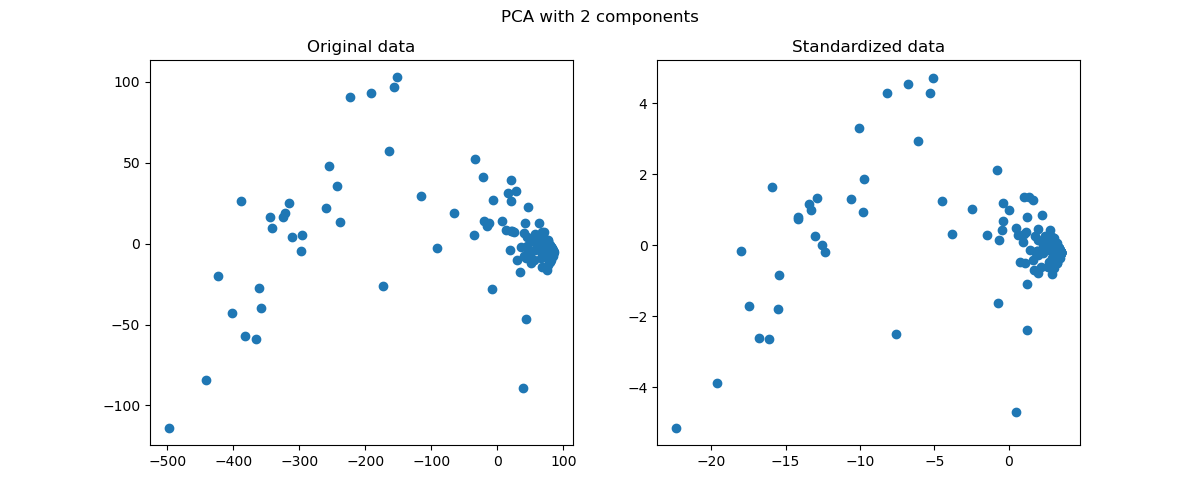
\includegraphics[width=1.0\linewidth]{reports/assignment-4/imgs/pca.png}
    \caption{Task 1 visualization (a)}
    \label{fig:pca}
\end{figure}

Figure \ref{fig:pca} shows a PCA performed on the original data and the standardized data. Both PCAs were done using the number of columns, i.e. 39, components, and the 2 dimensions accounting for the most variance are visualized. The PCA reduces the column dimensionality (years) into two components, which are then plotted. The plots themselves are almost similar, but the standardized plot has a much smaller range of values on both axes. The plots show a small cluster on the right-hand-side, and the rest of the countries are pretty scattered around the value space.

\begin{figure}[h!]
    \centering
    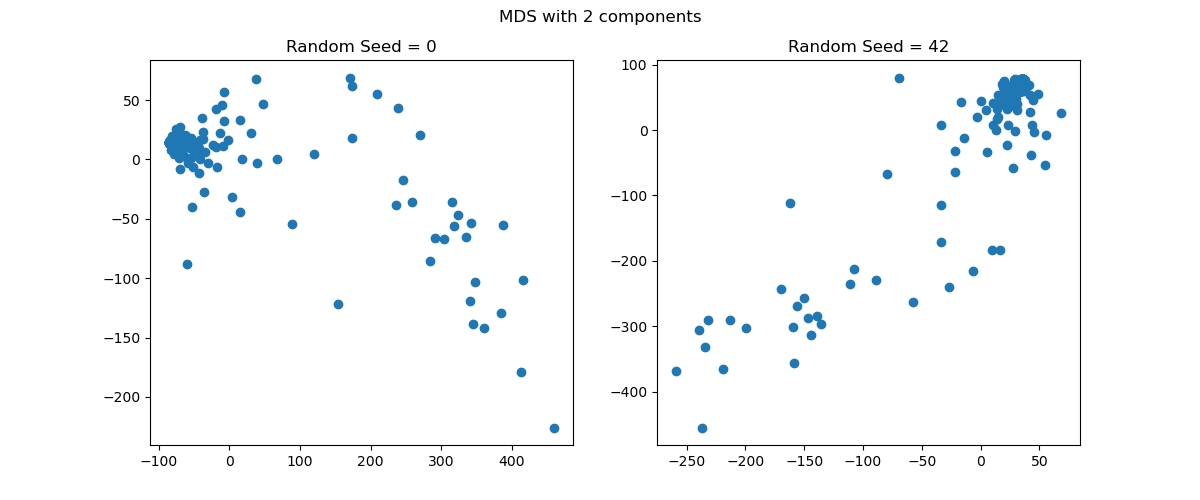
\includegraphics[width=1.0\linewidth]{reports/assignment-4/imgs/mds.png}
    \caption{Task 1 visualization (b)}
    \label{fig:mds}
\end{figure}

\newpage

Figure \ref{fig:mds} shows an MDS using two components performed on the dataset with two different random seeds for initialization. Both plots show a large cluster of points, which means that many of the countries are similar in their development over the years (the Euclidean distance between two row vectors is fairly small). This cluster is most likely the countries that have a large share of poverty in the beginning of the time interval and in the end, since they are largest in number in the dataset. Then, the points closer to the cluster but clearly outside it are the countries that have had a change in the poverty share over the years, and lastly the points furthest away from the cluster are the points that have had a relatively low share of poverty throughout the time interval.

\begin{figure}[h!]
    \centering
    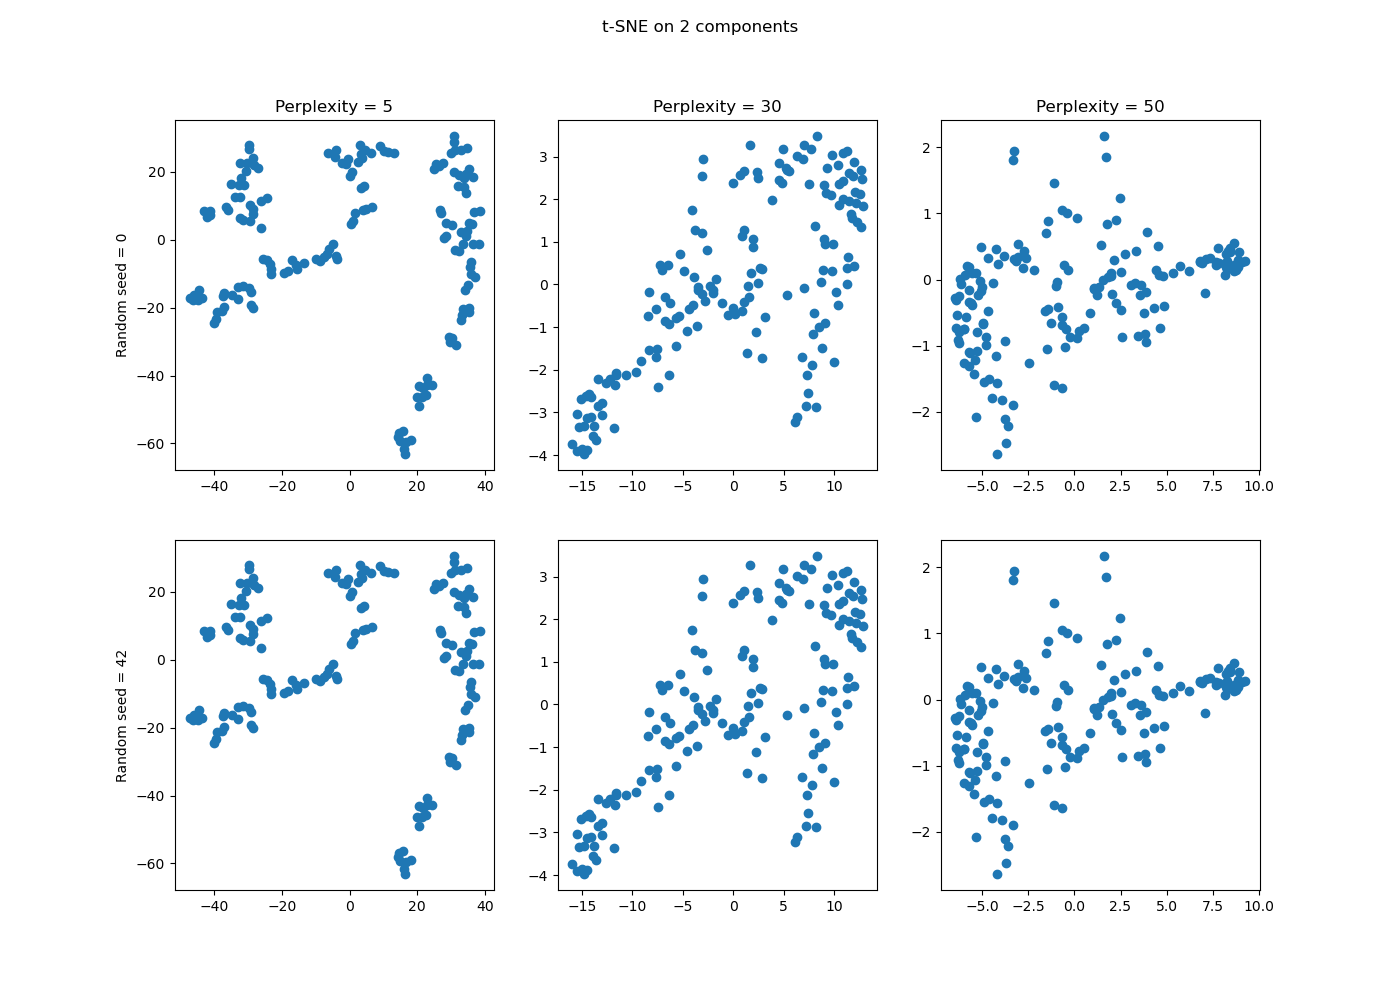
\includegraphics[width=1.0\linewidth]{reports/assignment-4/imgs/tsne.png}
    \caption{Task 1 visualization (c)}
    \label{fig:tsne}
\end{figure}

\newpage

Figure \ref{fig:tsne} shows a t-SNE performed on the data using 6 different initializations. Each t-SNE was initialized with 2 components, initialization method set to random, and perplexity and seed to the values shown in the visualization. As can be seen in the plots, perplexity values of 30 and 50 are far too large, producing plots with no structure whatsoever. The plots with 5 perplexity however, show 3-4 small clusters in them, suggesting similarity between countries.

Working on this task, I encountered some problems that arose mostly due to my lack of experience with these dimensionality reduction methods. At first, it was difficult to produce meaningful plots using the methods, and after that, I had difficulty interpreting the plots. Reading the methods' Wikipedia pages helped me understand the methods better, enabling me to analyze the plots better.

\section{Relational Data}

In this task, I produced visualizations portraying the relationships between datapoints. I produced 5 different graph visualizations portraying the interconnections between the SDGs. For this reason, I first had to make an adjacency matrix. I constructed the matrix by first going over each relationship, and deciding whether there is a clear and strong connection between the SDGs. For example, the SDGs "No Poverty" and "Zero Hunger", are in my opinion very strongly connected, thus they share an edge. In the beginning, I had way too many connections, and I had to prune them by going over them again. I decided that to maintain some balance in the plot, each node could be connected to 5 other nodes maximum. This helped pruning the connection space, resulting in a fairly balanced adjacency matrix.

\begin{table}[h!]
    \centering
    \renewcommand{\arraystretch}{1}
    \scalebox{0.7}{\begin{tabular}{c|ccccccccccccccccc}
        & 1 & 2 & 3 & 4 & 5 & 6 & 7 & 8 & 9 & 10 & 11 & 12 & 13 & 14 & 15 & 16 & 17 \\ \hline
      1  & 0 & 1 & 1 & 1 & 0 & 1 & 0 & 0 & 0 & 1 & 0 & 0 & 0 & 0 & 0 & 0 & 0 \\
      2  &   & 0 & 1 & 0 & 0 & 1 & 0 & 0 & 0 & 1 & 0 & 0 & 0 & 0 & 0 & 0 & 0 \\
      3  &   &   & 0 & 1 & 0 & 1 & 0 & 0 & 0 & 0 & 0 & 0 & 0 & 0 & 0 & 0 & 1 \\
      4  &   &   &   & 0 & 1 & 0 & 0 & 1 & 1 & 0 & 0 & 0 & 0 & 0 & 0 & 0 & 0 \\
      5  &   &   &   &   & 0 & 0 & 0 & 1 & 0 & 1 & 0 & 0 & 0 & 0 & 0 & 0 & 1 \\
      6  &   &   &   &   &   & 0 & 0 & 0 & 0 & 1 & 0 & 0 & 0 & 0 & 0 & 0 & 0 \\
      7  &   &   &   &   &   &   & 0 & 0 & 0 & 0 & 1 & 1 & 1 & 1 & 1 & 0 & 0 \\
      8  &   &   &   &   &   &   &   & 0 & 1 & 0 & 0 & 1 & 0 & 0 & 0 & 0 & 0 \\
      9  &   &   &   &   &   &   &   &   & 0 & 0 & 1 & 0 & 0 & 0 & 0 & 0 & 0 \\
     10  &   &   &   &   &   &   &   &   &   & 0 & 0 & 0 & 0 & 0 & 0 & 0 & 1 \\
     11  &   &   &   &   &   &   &   &   &   &   & 0 & 0 & 0 & 0 & 1 & 0 & 0 \\
     12  &   &   &   &   &   &   &   &   &   &   &   & 0 & 1 & 1 & 1 & 0 & 0 \\
     13  &   &   &   &   &   &   &   &   &   &   &   &   & 0 & 1 & 1 & 0 & 1 \\
     14  &   &   &   &   &   &   &   &   &   &   &   &   &   & 0 & 1 & 0 & 0 \\
     15  &   &   &   &   &   &   &   &   &   &   &   &   &   &   & 0 & 0 & 0 \\
     16  &   &   &   &   &   &   &   &   &   &   &   &   &   &   &   & 0 & 1 \\
     17  &   &   &   &   &   &   &   &   &   &   &   &   &   &   &   &   & 0 \\
    \end{tabular}
    }
    \caption{Adjacency matrix of SDGs}
    \label{adj}
\end{table}

The adjacency matrix is found in table \ref{adj}. In the table, the row and column numbers denote the SDG number given by United Nations. The value of a cell is 1 if there is an edge between the nodes, and 0 otherwise. Each visualization in this task was made using \texttt{networkx} and \texttt{matplotlib}. \texttt{networkx} was used to initialize and structure the graphs and assign layouts to them, while \texttt{matplotlib} was used to create the plots. In each plot, the number inside the node denotes the SDG it is.

\newpage

\begin{figure}[h!]
    \centering
    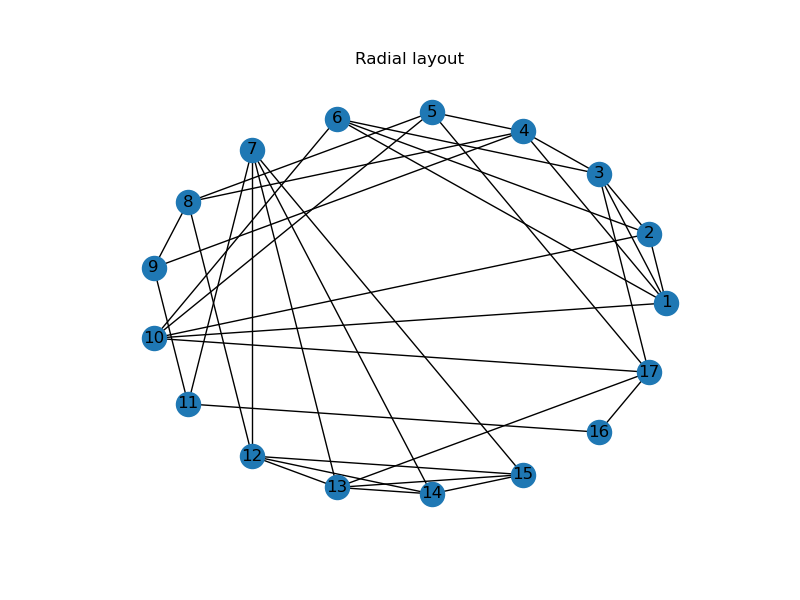
\includegraphics[width=0.8\linewidth]{reports/assignment-4/imgs/radial.png}
    \caption{Task 2 visualization (a)}
    \label{fig:rad}
\end{figure}

Figure \ref{fig:rad} shows a plot of the adjacency matrix with a radial layout and numerical ordering. In my opinion, this layout makes finding nodes and fetching connections between nodes very easy and efficient. However, there are shortcomings to this layout, since finding, for example, cliques is very laboursome.

\begin{figure}[h!]
    \centering
    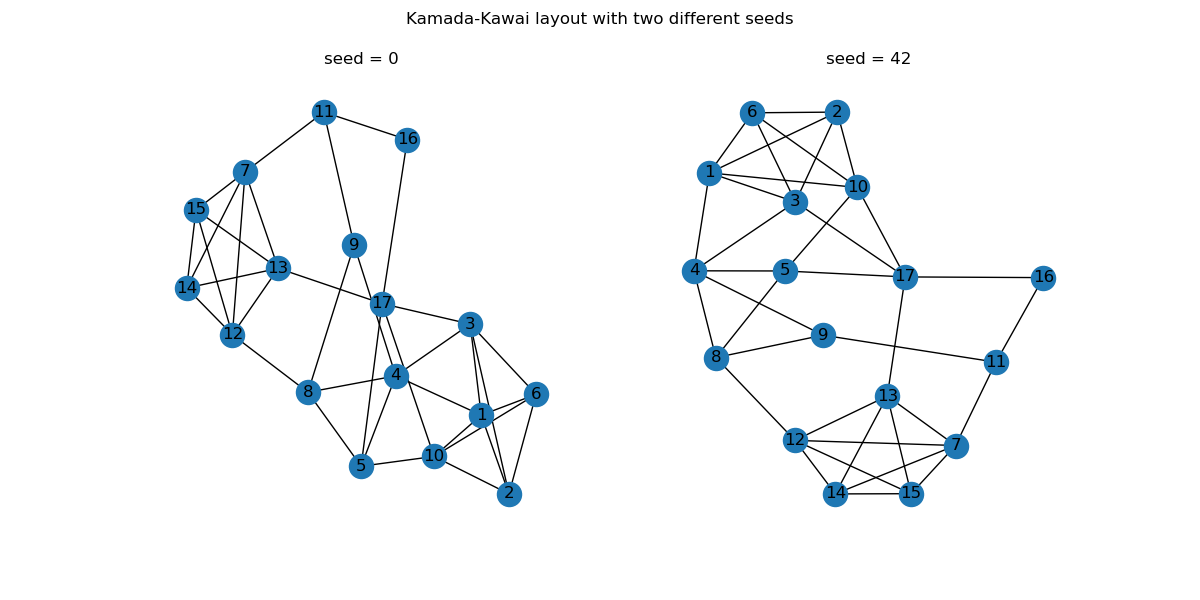
\includegraphics[width=1.0\linewidth]{reports/assignment-4/imgs/kk.png}
    \caption{Task 2 visualization (b)}
    \label{fig:kk}
\end{figure}

Two different Kamada-Kawai layouts are visualized in figure \ref{fig:kk}. A different random seed, producing a random initial layout, was used for both visualizations. This layout makes finding smaller subgraphs within the graph easy, but finding individual nodes is a bit harder because of the unordered nature of the layout. There are a lot less crossing edges than in the radial layout, making the plots a lot cleaner in my opinion.

\begin{figure}[h!]
    \centering
    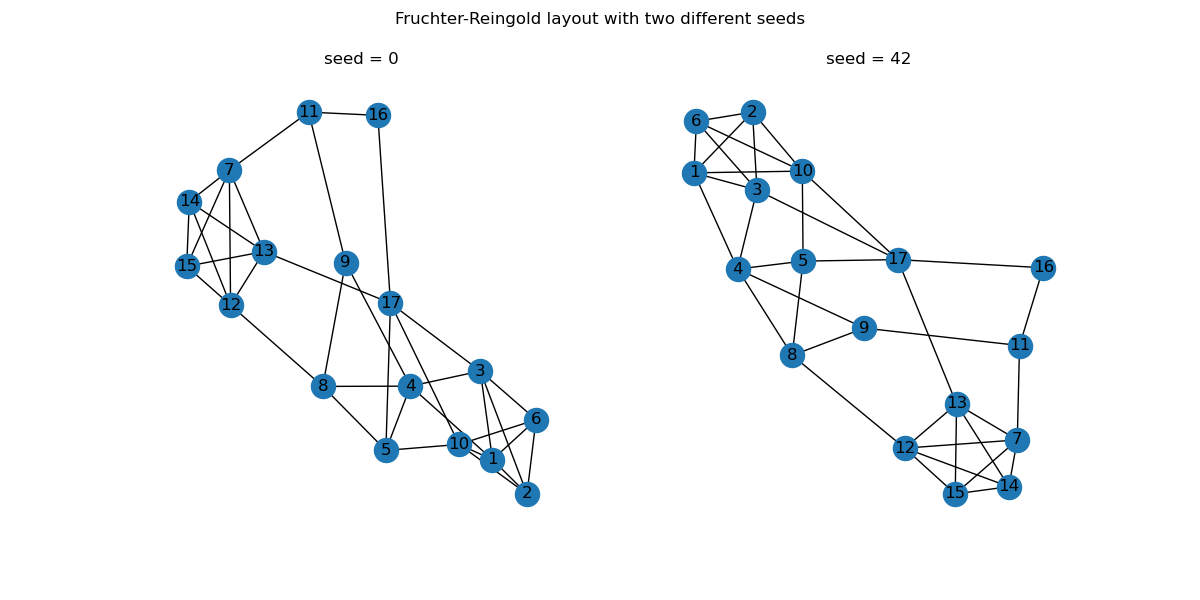
\includegraphics[width=1.0\linewidth]{reports/assignment-4/imgs/fr.png}
    \caption{Task 2 visualization (c)}
    \label{fig:fr}
\end{figure}

Figure \ref{fig:fr} shows two different graph visualizations using a Fruchterman-Reingold layout. The plots, like the Kamada-Kawai ones, were obtained using two different random seeds, producing similar, but still different positions for the nodes. The plots are very similar to the Kamada-Kawai plots, an as such, the same observations and notes apply to these plots as well.

As \texttt{networkx} is a fairly new library to me, I had some troubles working with it. The majority of my headaches were caused by trying to create the Kamada-Kawai and Fruchterman-Reingold layouts using the randomization. Neither of the \texttt{networkx} functions for creating the layouts had a random seed as a parameter, so in the beginning, I was a bit stumped. After a bit of searching and reading the documentation, I found a function used for creating a random layout. I used this function for initializing the positions of the nodes, then passing the initial position to the layout function. This resulted in different and reproducible visualizations for different random seeds.

\newpage

\bibliography{reports/assignment-4/refs}

\end{document}